\documentclass{HW}

\newcommand{\hwtitle}{آزمایش دو}
\newcommand{\studentname}{رادین شایانفر}
\newcommand{\studentnumber}{9731032}

\usepackage[top=30mm, bottom=30mm, left=25mm, right=25mm]{geometry}
\usepackage{amsthm,amssymb,amsmath,amsfonts}
\usepackage{fancyhdr}
\usepackage{changepage}
\usepackage{enumitem}
\usepackage{listings}
\usepackage[table]{xcolor}
\usepackage{fontspec}

\newfontfamily{\ttconsolas}{Consolas}

\definecolor{codegreen}{rgb}{0,0.6,0}
\definecolor{codegray}{rgb}{0.5,0.5,0.5}
\definecolor{codepurple}{rgb}{0.58,0,0.82}
\definecolor{backcolour}{rgb}{0.95,0.95,0.92}

\lstset{
  backgroundcolor=\color{backcolour},   
  commentstyle=\color{codegreen},
  keywordstyle=\color{magenta},
  numberstyle=\tiny\color{codegray},
  stringstyle=\color{codepurple},
  basicstyle=\ttconsolas\footnotesize,
  breakatwhitespace=false,         
  breaklines=true,                 
  captionpos=b,                    
  keepspaces=true,  
  numbers=left,                    
  numbersep=5pt,                  
  showspaces=false,                
  showstringspaces=false,
  showtabs=false,                  
  tabsize=4
}

\usepackage{array,multirow}

\usepackage{tikz}
\usetikzlibrary{trees}

% بسته‌‌ای برای ظاهر شدن شکل‌ها و تصاویر متن
\usepackage{graphicx}
\usepackage{color}
%بسته‌ای برای تنظیم فاصله عمودی خط‌های متن
\usepackage{setspace}

\usepackage[pagebackref=false,colorlinks,urlcolor=cyan,linkcolor=blue,citecolor=red]{hyperref}

\hypersetup{
    pdftitle={\hwtitle - \studentname - شماره دانشجویی: \studentnumber},
    bookmarks=true,
    pdfauthor={Radin Shayanfar},
}

% بسته‌ لازم برای تنظیم سربرگ‌ها
\usepackage{fancyhdr}

\usepackage{ptext} 
\usepackage{xepersian}

\doublespacing

\SepMark{-}
\settextfont[Scale=1.2]{B Nazanin}
\setlatintextfont{Times New Roman}
\renewcommand{\labelitemi}{$\bullet$}

\newcounter{mynumber}
\setcounter{mynumber}{1}
\newcommand{\mynum}{\arabic{mynumber}\stepcounter{mynumber}}

\newenvironment{question}{%
\medskip%
\par%
\noindent%
\textbf{سوال \mynum- \space}%
\smallskip
%\par\noindent\ignorespaces
\begin{adjustwidth}{7mm}{}
}{%
\end{adjustwidth}
\par\medskip
}

\fancypagestyle{first_page}{
\fancyhf{}
\fancyhead[C]{\raisebox{3ex}{\large \bfseries \hwtitle}}
\fancyhead[LO,LE]{\textbf{\studentname} \\
شماره دانشجویی: \studentnumber
\vspace{0.2mm}}
\fancyfoot[C]{\thepage{}}
\renewcommand{\headrulewidth}{1.2pt}
}

\fancypagestyle{pages}{
\fancyhf{}
\fancyhead[R]{\leftmark}
\fancyfoot[C]{\thepage{}}
\renewcommand{\headrulewidth}{1.2pt}
}

\begin{document}
\pagestyle{pages}
\thispagestyle{first_page}

\section{مرحله اول}

ابتدا تغییراتی در کد برنامه سریال می‌دهیم و امکاناتی مانند اندازه‌گیری زمان اجرا و زمان میانگین چند اجرا را به آن اضافه می‌کنیم. پس از انجام این تغییرات، برنامه را به صورت سریال اجرا می‌کنیم. یک نمونه از اجرای کد سریال را برای ماتریس ۸ در ۸ در شکل
\ref{fig:serial}
می‌بینیم.

\begin{figure}[ht!]
\begin{center}
	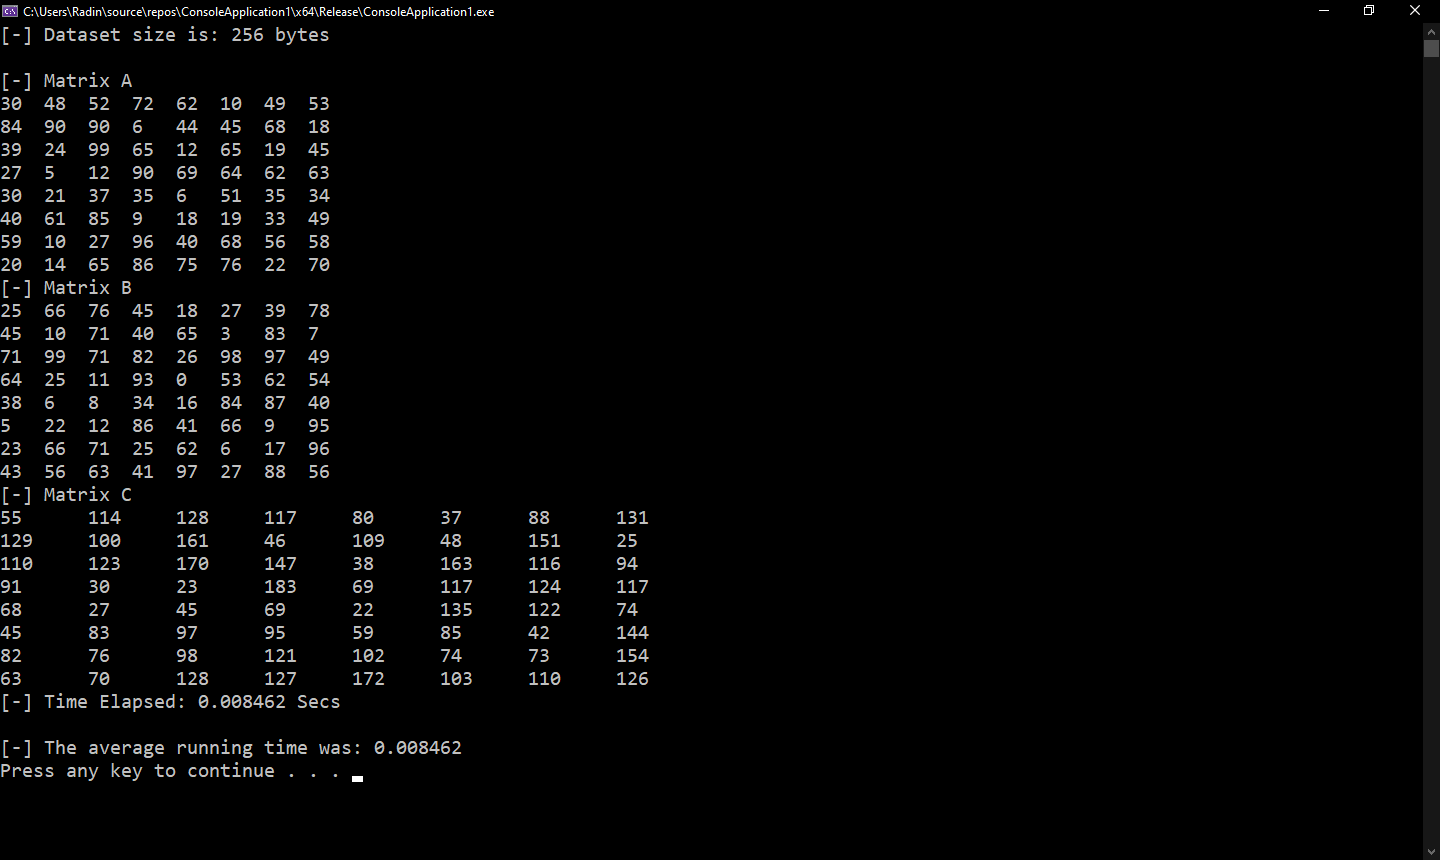
\includegraphics[width=15cm]{images/serial}
\end{center}
\caption{نمونه اجرای کد سریال}
\label{fig:serial}
\end{figure}

\section{مرحله دوم}

برای تجزیه یک بعدی، با استفاده از راهنمای زیر، می‌توانیم اجراهای حلقه بیرونی را موازی کنیم. همچنین برای بهتر دیدن تجزیه، شماره نخ را به جای جمع ماتریس‌ها داخل ماتریس خروجی می‌نویسیم. حاصل نوشتن شماره نخ داخل ماتریس خروجی را در شکل
\ref{fig:1d-decomp-thnum}
می‌بینیم.
\textbf{پس از اطمینان از درستی تجزیه، جهت اندازه‌گیری درست زمان اجرا مجدد برنامه را به حالت قبلی (جمع ماتریس) برمی‌گردانیم.}
همچنین یک نمونه از جمع صحیح دو ماتریس با تجزیه یک بعدی در شکل
\ref{fig:1d-decomp-add}
نشان داده شده است.

\begin{latin}
\begin{minipage}{\linewidth}
\begin{lstlisting}[language=C]
#pragma omp parallel for
for (i = 0; i < dataSet.n; i++) {
	for (j = 0; j < dataSet.m; j++) {
		dataSet.C[i * dataSet.m + j] = omp_get_thread_num();
	}
}
\end{lstlisting}
\end{minipage}
\end{latin}

\begin{figure}[ht!]
\begin{center}
	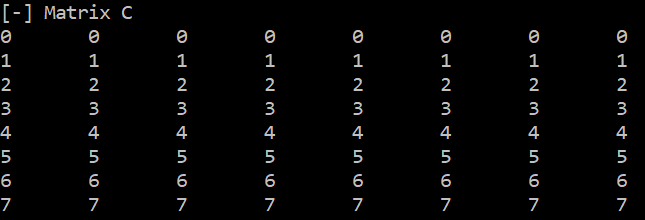
\includegraphics[width=12cm]{images/1d-decomp-thnum}
\end{center}
\caption{نحوه تخصیص نخ‌ها در حالت تجزیه یک بعدی برای یک ماتریس ۸ در ۸}
\label{fig:1d-decomp-thnum}
\end{figure}

\begin{figure}[ht!]
\begin{center}
	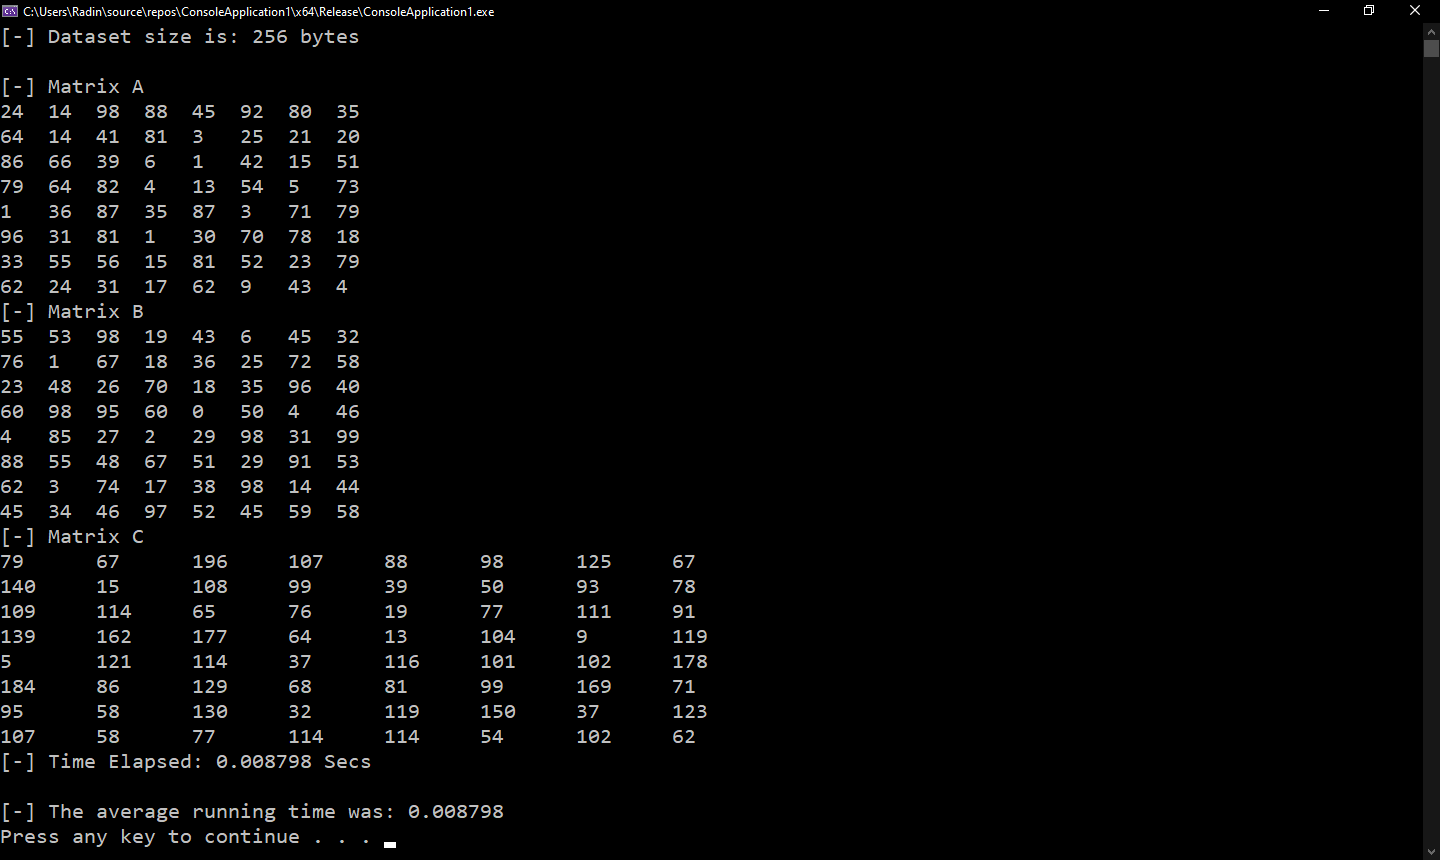
\includegraphics[width=15cm]{images/1d-decomp-add}
\end{center}
\caption{یک نمونه از جمع ماتریس با تجزیه یک بعدی}
\label{fig:1d-decomp-add}
\end{figure}

\section{مرحله سوم}


\begin{table}[ht]
\caption{نتایج روش اول}
\begin{center}
\begin{tabular}{|c|c|c|c|c|c|}
    \hline
    \multirow{2}{*}{تعداد نخ‌ها} & \multicolumn{4}{|c|}{میانگین زمان اجرا (ثانیه)}& \multirow{2}{*}{تسریع} \\
    \cline{2-5}
& \lr{1MB} & \lr{10MB} & \lr{100MB} & \lr{1GB} & \\
    \hline
  1 & 0/010209 & 0/103059 & 1/074217 & & \\ \hline
  2 & 0/014540 & 0/120412 & & & \\ \hline
  4 & 0/015604 & 0/138814 & & & \\ \hline
  8 & 0/025209 & 0/184495 & 1/277460 & & \\ \hline
\end{tabular}
\end{center}
\label{tab:1d}
\end{table}


\end{document}
